\chapter{Le NoSQL dans les SIG}

\section{Les Systèmes d’Information Géographiques}
\subsection{Définition}
\paragraph{}Un système d'information géographique est un système d’information permettant, à partir de plusieurs sources de données, de recueillir, stocker, traiter, analyser, gérer et présenter des données à la fois spatiales et géographiques. Les \acrshort{SIG}, avec d’autres traitements, font partie du domaine de la géomatique. 

\paragraph{}Comme tout système d’information, le \acrshort{SIG} offre un soutien aux processus de travail. Il permet d'analyser spatialement un phénomène tout en fournissant l'information et automatisant le travail humain.

\subsection{Historique}
\paragraph{}Les années 1960 correspondent au début des \acrfull{SIG}. Avec l’apparition des ordinateurs, les premiers travaux de recherches sont apparus sur des sujets comme l’analyse spatial et la visualisation de l’information géographique, constituant donc les bases des \acrshort{SIG}. Auparavant, diverses analyses spatiales ont pu être effectuées en France ou au Royaume-Uni comme celle concernant les effets du choléra dans l’ancien département de la Seine \footnote{ancien département comprenant Paris et une partie des communes des Hauts-de-Seine, de Seine-Saint-Denis et du Val-de-Marne} en 1832 \supercite{rapportCholeraSeine}. Toutefois, c’est le développement de l’informatique dans la deuxième partie du XXème siècle qui a permis le développement des \acrshort{SIG} en tant que tel.
\paragraph{}En 1963, Robert Tomlinson \supercite{tomlinson} a mis en place un outil permettant de regrouper des données sur l’inventaire des ressources naturelles et sols canadiens et cela constitue le premier \acrshort{SIG}. En parallèle, Howard Fisher a créé le premier logiciel de cartographie informatique, nommé SYMAP. En 1965, il crée le Laboratoire de Harvard pour l'infographie et l'analyse spatiale où seront conçus les premiers concepts et applications dans ce domaine. Ces recherches ont permis le développement de systèmes dans les années 1970, utilisés par les universités, les centres de recherche et des entreprises.

\paragraph{}Le \acrshort{SIG} canadien a servi de base de travail jusqu’en 1986 où le premier \acrshort{SIG} à usage personnel a été créé : le système MIDAS (Mapping Display and Analysis System). Par la suite, le développement à la fois des systèmes d’information et d’Internet ont permis la démocratisation des \acrshort{SIG}. C’est à ce moment, en 1994, que l’Open Geospatial Consortium a été créé par promouvoir des standards liés à l’information géographique et la géomatique afin de permettre l’interopérabilité des contenus et échanges. Plus récemment, les solutions Open Source ont permis de rendre ces technologies plus accessibles.

\paragraph{}Depuis, nombre d'entre eux sont utilisés dans divers domaines allant de la cartographie avec les services de géolocalisation à l'analyse de situations telles que les élections, les déplacements de populations ou les épidémies à l'instar des outils réalisés suite à la pandémie de COVID-19 :
\begin{figure}[htp]
  \centering
  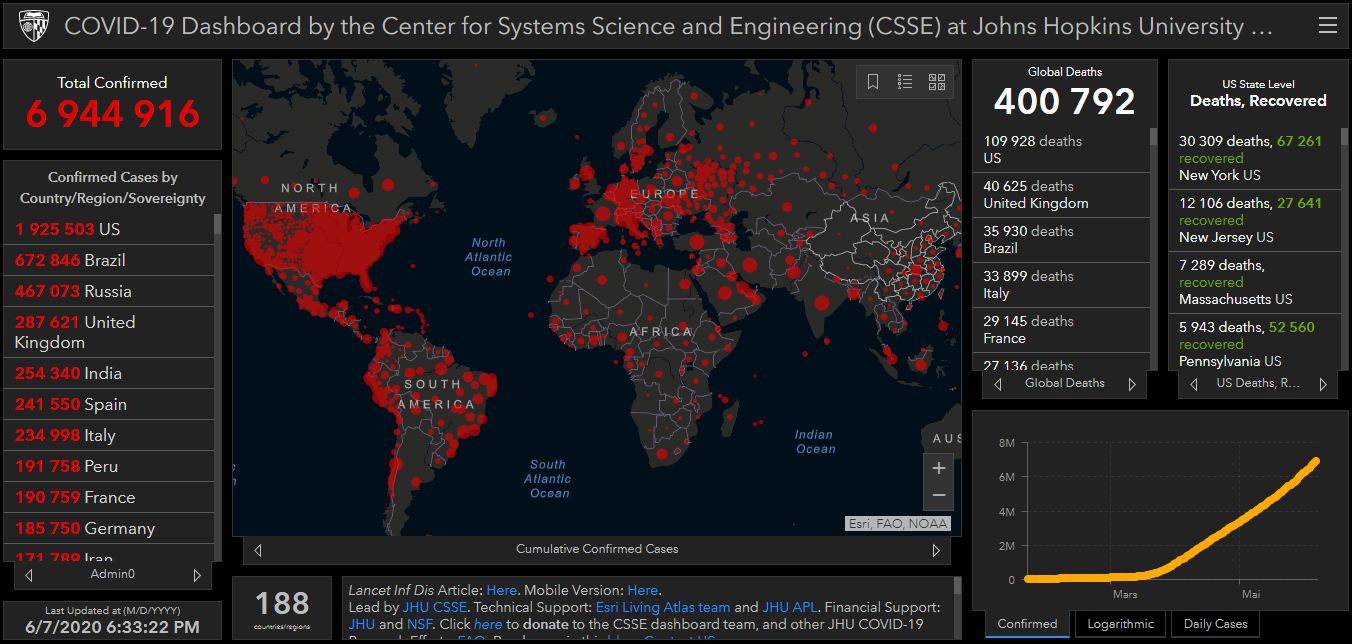
\includegraphics[width=120mm]{src_img/gis_use_example.png}
  \caption{Utilisation d'ArcGIS (un \acrshort{SIG}) dans le cadre de l'épidémie de Covid-19\supercite{arcgisCovid}}
  \label{fig:arcgisexemple}
\end{figure}

\subsection{Les composants}
Pour réaliser tout ce qui lui est induit, les systèmes d’information géographiques sont composés \supercite{giscomponents} de :
\begin{description}
    \item[matériel informatique :] les \acrshort{SIG} fonctionnent sur une large gamme de matériel, de serveurs informatiques centralisés aux ordinateurs de bureau utilisés dans des configurations autonomes ou en réseau
    \item[logiciels :] ils fournissent les outils nécessaires pour sauvegarder, traiter et visualiser l’information géographique contenue dans des bases de données
    \item[données :] l’information géographique est la pièce maîtresse des \acrshort{SIG}. Elle peut être récupérée ou constituée
    \item[personnel :] les outils nécessitent des personnes chargées de manipuler et traiter l’information géographique. La démocratisation des \acrshort{SIG} a permis l’augmentation du nombre d’utilisateurs
\end{description}

\subsection{Les principes des SIG}

Ces composants ensemble permettent de suvre les principes des “5A” :
\begin{description}
    \item[L’acquisition :] Elle correspond à obtenir et regrouper différentes sources afin de les intégrer au SIG selon le problème à résoudre. Les sources sont diverses (visites de terrain, satellite, etc.)
    \item[L’archivage :] Consiste à réaliser un choix concernant le stockage et le traitement des données, organisé par thématique (ex: voirie, occupation des sols)
    \item[L’accès :] Mise à disposition des données d’information (données et cartes) et de les combiner
    \item[L’analyse :] Correspond aux possibilités offertes par le SIG pour traiter les données au travers d’outils grâce à des mesures, des calculs ou des requêtes spatiales
    \item[L’affichage :] Correspond en la restitution cartographique des données correspondant au besoin spécifique
\end{description}

\paragraph{}Un sixième aspect est également parfois cité, l’abstraction \supercite{courssig}. Cet aspect correspond à permettre la conception d'un modèle arrangeant les données par constituants géométriques et attributs descriptifs tout en établissant les relations entre les objets.


\subsection{Les données}
Les \acrshort{SIG} se basent sur deux types de données qui se complètent : spatiales et attributaires.

\subsubsection{Données spatiales}

Un Système d’information Géographique s’appuie sur un modèle de couches organisé de manière cohérente afin de décrire et caractériser le plus fidèlement le monde. Par exemple, un SIG peut avec comme couches la topologie \footnote{étude des déformations du sol}, les réseaux hydrographiques ou de communication ou le découpage et l'occupation des sols.

Deux formats permettent de stocker les données spatiales (99\% des SIG savent traiter les deux types) :

\begin{itemize}[label=\textbullet]
    \item Le format raster, ou maillé, a une géométrie fondée sur un découpage en mailles élémentaires, de la même façon qu’une image numérique est découpée en pixels. L’information spatiale apparaît sous la forme d’un tableau de valeurs numériques référencées géographiquement.
    \item Les vecteurs ont une géométrie fondée sur un système de coordonnées vectorielles assimilables au dessin classique d’une carte traditionnelle. Les objets spatiaux sont représentés par des points, des arcs ou des polygones, et la position des objets est donnée par rapport à un repère standard (géographique ou cartésien).
\end{itemize}
\begin{figure}[htp]
  \centering
  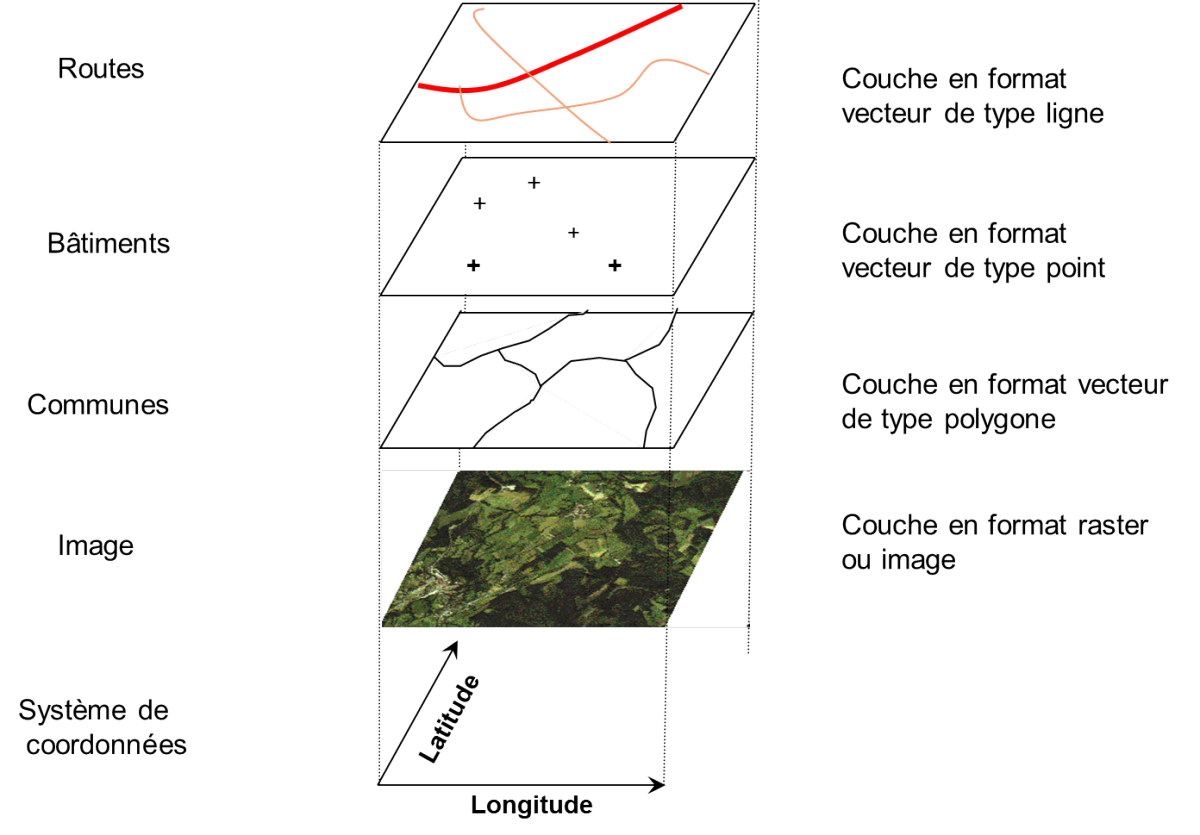
\includegraphics[width=90mm]{./src_img/structure_donnees.png}
  \caption{Exemple de couches \supercite{uved}}
  \label{fig:struct}
\end{figure}
Comme il est possible de voir sur le schéma de la figure \ref{fig:struct}, la représentation d'une situation géographique correspond souvent à l'utilisation des deux formats présentés. Pour leur stockage, il est réalisé par le biais d'arbres et de graphes \supercite{arbresSIG} qui permettent d'équilibrer les données.

%Sur l'exemple ci-dessus (figure \ref{fig:struct}), les différentes couches et formats présentés juste avant.

%Les SIG possèdent des données spatiales qui peuvent être stockées soit en format vectoriel, soit en format raster. Le vectoriel va gérer les points, les lignes et les polygones alors que le raster va utiliser une photographie aérienne, une carte ou une image satellite pour la découper sous forme d'une matrice. Cette matrice de cellules (ou pixels) est elle-même organisée sous forme de grille. Ces données spatiales, qu'elles soient sous format vecteur ou raster, sont complétées par des données alphanumériques. Leur stockage est réalisé avec l'utilisation d'arbres et de graphes \supercite{arbresSIG} qui permettent d'équilibrer les données.
%Par exemple, un SIG peut distinguer parcelles, images satellites, réseau hydrographique et bâtiments sur une zone d’intérêt.

\subsubsection{Données associées}
\paragraph{}Ces données permettent, avec la topologie \footnote{topologie : décrit les relations entre objets}, de compléter l’information spatiale \supercite{courssig2} comme il est possible de voir dans la figure \ref{fig:besoinSpatial}. Elles constituent en quelque sorte l’étiquette permettant de donner des détails sur un point, une ligne ou un polygone. Parmi les données associées :
`\begin{itemize}[label=\textbullet]
    \item les données de classification : elles permettent de classer la forme selon des classes déterminées, par exemple si une route est primaire ou secondaire ou si une parcelle est irriguée ou non
    \item les données d’identification : ce sont les informations distinguant un objet d’un autre comme le nom de la commune, le numéro de parcelle
    \item les données attributaires  : c’est une information complémentaire propre à l’objet (ex : propriétaire, superficie)
\end{itemize}

\begin{figure}[htp]
  \centering
  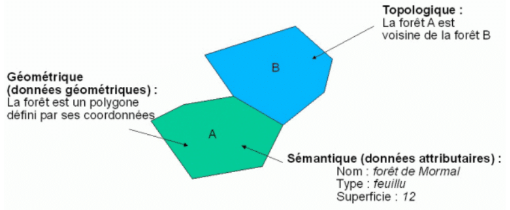
\includegraphics[width=95mm]{src_img/exempleBDS.png}
  \caption{Les 3 niveaux de la donnée géographique \supercite{ensg}}
  \label{fig:besoinSpatial}
\end{figure}

\section{Quelles différences entre SQL et NoSQL ?}

\subsection{Les bases de données relationnelles}

\paragraph{}Les bases de données relationnelles utilisent un modèle établit par Edgar F. Codd en 1970. Dans ce modèle, l’information est organisée dans des tableaux à deux dimensions, appelées relations ou tables et faisant correspondre ces données selon des caractéristiques communes. Chaque table est donc structurée par un schéma préconçu.

\paragraph{}Codd a également établit le langage\newacronym{SQL}{SQL}{Structured Query Language} \acrshort{SQL}, permettant de créer le schéma et les données mais également d’interroger la base de données, y compris des opérations d’intersection, de sélection ou de jointure. Il est utilisé par les différents \acrlong{SGBD} relationnels tels que Oracle, Sybase, Microsoft SQL Server ou Access.

\subsubsection{Propriétés}
\paragraph{}Les SGBD relationnels suivent les propriétés ACID :
\begin{description}
    \item[Atomicité :] signifie «tout ou rien». Si une partie de la transaction reste incomplète, la transaction entière est considérée comme ayant échoué.
    \item[Cohérence:] garantit qu'une base de données avant et après toute transaction est stable à un état valide.
    \item[Isolation:] garantit que plusieurs transactions exécutées en même temps n'affectent pas l'exécution de l'autre, cela nécessitant la sérialisation des transactions simultanées
    \item[Durabilité:] garantit qu'une fois qu'une transaction a été validée, elle reste dans le même état, c'est-à-dire qu'elle stocke en permanence même en cas d'erreurs, de panne du système ou de coupure de courant
\end{description}

\subsection{Les bases de données NoSQL}

\paragraph{}Les bases de données NoSQL (“Not only SQL” ou “pas seulement SQL”) sont apparus à la fin des années 2000 avec le développement des centres de données et la nécessité d’avoir un paradigme adapté à une architecture en clusters, donc distribuée. Cette architecture apporte aussi la possibilité d’accès et modifications concurrentes, non permises par les propriétés ACID des SGBD relationnels. Elle est également auto-descriptive et ne nécessite donc pas de schéma.

\paragraph{}Afin de répondre à des volumes de plus importants (comme le Big Data) et leur besoin de gérer des données distribuées, certaines entreprises du web ont créé leurs propres \acrshort{SGBD} : BigTable pour Google, MongoDB sur SourceForge.net et Cassandra puis HBase pour Facebook. Ces solutions sont devenus de plus en plus adoptées lors de la dernière décennie. 

\subsubsection{Propriétés}
\paragraph{}Associé au développement des systèmes distribués, un nouveau concept opposé à ACID est apparu, le concept BASE :
\begin{description}
    \item[Basic Availability :] le système doit à tout moment  être accessible.
    \item[Soft state :] l'état de la base de données n'est pas garanti à un instant t.
    \item[Eventually Consistent :] la cohérence des données à un instant t n'est pas primordiale.
\end{description}

\subsubsection{Diffférents modèles existants}
\begin{description}
    \item[Clé-valeur \supercite{NoSQLModels} :] le modèle de données basé sur un tableau associatif dans lequel les données sont représentées sous une collection de paires clé-valeur. Ils conviennent parfaitement à la gestion de session et à la mise en cache dans les applications Web (utilisé par LinkedIn)\\
    Exemples: Aerospike,  Redis, Riak\\
    \item[Colonne :] une large colonne stocke et organise les tableaux de données sous forme de colonnes plutôt que de lignes. Cette structure permet d’interroger rapidement un grand volume de données comme pour les moteurs de recommandation, les catalogues, la détection de fraude, etc. (Utilisé par Amazon, Google et Facebook) \\
    Exemples: Cassandra, HBase, Google BigTable\\
    \item[Document :] ce modèle conserve les données semi-structurées ainsi que leur description au format du document (souvent XML ou JSON). Chaque document possède une clé unique à travers laquelle il est adressé. Ils sont particulièrement pour la gestion de contenus et de données des applications mobile mais avec JSON et lors d’utilisations d’API. (Utilisé par Expedia, SAP et Salesforce) \\
Exemples: Apache, MongoDB, CouchDB, BaseX\\
    \item[Graphe :] les données sont organisées en nœuds (correspondant à un enregistrement) et en arêtes. Ce modèle prend en charge une représentation plus riche des relations de données. Ils sont utiles pour les systèmes de gestion de la relation client, les cartes routières, les systèmes de réservation, etc. (Utilisé par eBay et Accenture)\\
Exemples: AllegroGraph, InfiniteGraph,  Neo4j, Titan\\
\end{description}
\subsection{Des possibilités d'analyse sur plusieurs dimensions}
Nous avons pu voir que le choix de la structure est primordial dans la mise en place d'une base de données. Il est également nécessaire de penser à l'analyse qu'on ferait de son contenu. Pour répondre à des besoins de plus en plus importants concernant l'analyse sur plusieurs thématiques à la fois, l'analyse multidimensionnelle a été mise en place, en particuliers avec les technologies OLAP \footnote{OnLine Analytical Processing}.

\begin{figure}[!htp]
  \centering
  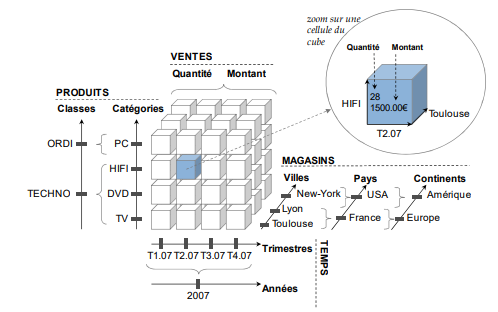
\includegraphics[width=75mm]{./src_img/exempleOLAPCube.png}
  \caption{Exemple de cube OLAP\supercite{tel-01456620}}
  \label{fig:olapcube}
\end{figure}

\paragraph{}Nous pouvons voir avec le cube de la figure \ref{fig:olapcube} qu'une des dimensions concerne des données géographiques, les villes. Le cube permet, par des opérations simples que sont le "drill-up" et le "drill-down" de remonter ou descendre la hiérarchie d'une dimension, par exemple accéder au niveau régional ou national des données.

\paragraph{}Toutefois, pour obtenir un cube que celui-là, il faut travailler à la conception de l'entrepôt de données dans lequel sont basées toutes les informations que l'on souhaite utiliser. Trois modèles existent dont un qui reprend les précédents :
\begin{itemize}[label=\textbullet]
    \item le modèle en étoile (figure \ref{Fig:modeletoile}) : il comprend une table de fait centrale avec des mesures qui sont dépendantes des différentes dimensions autour. Souvent sont utilisées une dimension géographique et une dimension temporelle
    \item le modèle en flocon (figure \ref{Fig:modelflocon}) : tout comme le modèle en étoile, il comprend une table de fait et des dimensions mais à l'instar d'un flocon de neige, ces dimensions ont des ramifications avec les hiérarchies sous-jacentes
    \item le modèle en constellation : il reprend les principes soit du modèle en étoile, soit du modèle en flocon mais à la différence qu'il comprend plusieurs tables de faits
\end{itemize}
\begin{figure}[!htb]
   \begin{minipage}{0.48\textwidth}
     \centering
     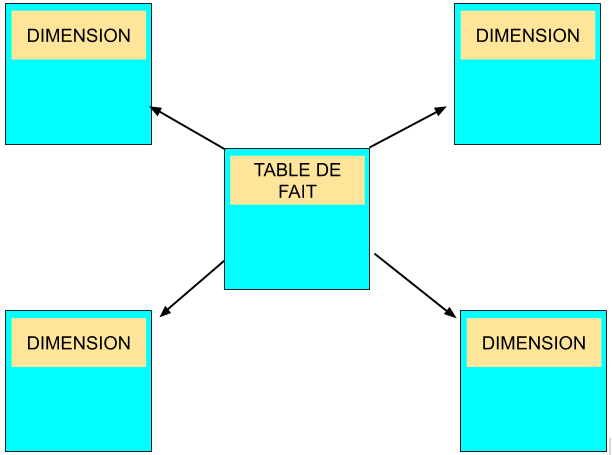
\includegraphics[width=.6\linewidth]{./src_img/Star-schema.png}
     \caption{Modèle en étoile}\label{Fig:modeletoile}
   \end{minipage}\hfill
   \begin{minipage}{0.48\textwidth}
     \centering
     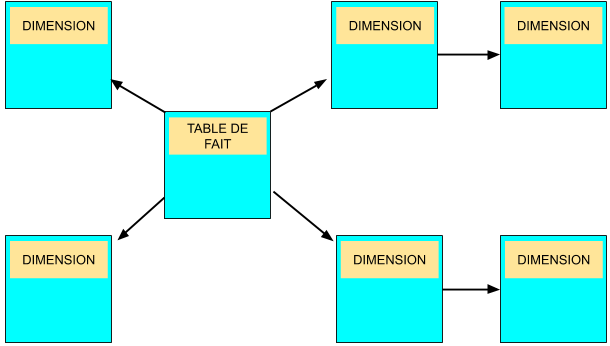
\includegraphics[width=.7\linewidth]{./src_img/SnowFlake-schema.png}
     \caption{Modèle en flocon}\label{Fig:modelflocon}
   \end{minipage}
\end{figure}
\paragraph{}Le modèle en étoile a par exemple l'avantage de permettre des requêtes plus simples, d'améliorer des performances des requêtes et l'alimentation d'un cube OLAP dont cette structure est privilégiée. A l'inverse, le modèle en flocon  permet d'avoir une structure plus normalisée  qui facilite donc l'ajout et surtout la mise à jour. En prenant l'exemple de la figure \ref{fig:olapcube}, les 2 modèles sont possibles. Cependant, pour l'utilisation d'un cube OLAP, le modèle en étoile est à privilégier.

Dans le cadre du NoSQL, à partir d'un document, d'une grosse colonne, plusieurs méthodes permettent de traduire la structure de données  \supercite{sgbd} :
\begin{itemize}[label=\textbullet]
    \item la traduction plate : l'ensemble des attributs de mesures et dimensions sont dans un même document
    \item la traduction par imbrication : les attributs et dimensions sont embriqués par catégorie dans le document
    \item la traduction hybride : les attributs et dimensions sont dans des documents différents avec des références entre eux
    \item la traduction éclatée : les attributs et dimensions sont dans des documents différents eux mêmes compris dans des collections
\end{itemize}
\paragraph{}Cette transformation permet ensuite une meilleure adaptabilité pour une utilisation dans un cube OLAP.

\subsection{Enoncé des différences notables}
\paragraph{}De nombreuses différentes entre SQL et NoSQL, à prendre à compte dans le choix d’un \acrshort{SGBD}. Les quatres principales distinctions sont :

\subsubsection{Le langage}
\paragraph{}Les SGBDR possèdent le SQL comme langage de requêtage. Sa structure, composée de schémas prédéfinis nécessite de déterminer la structure des données et donc une préparation initiale. Toutefois, cette structuration lui permet de mieux gérer les requêtes complexes. De leur côté, les bases de données NoSQL disposent d’un schéma dynamique. Cependant, les requêtes se basent sur \newacronym{UnQL}{UnQL}{Unstructured Query Language} \gls{UnQL} dont la syntaxe varie d'une base de données à l'autre.

\subsubsection{L’évolutivité}

\paragraph{}Dû à son architecture, les bases de données NoSQL peuvent plus facilement évoluer que les SQL et faire face à une augmentation du trafic. En effet, les SGBD relationnels, évolutifs verticalement, nécessitent d’augmenter la charge d’un seul serveur en augmentation ses composants (RAM, SSD, CPU) alors que le NoSQL nécessite uniquement l’augmentation du nombre de serveurs. De cette façon, le NoSQL est également plus résistant aux pannes et coûte donc moins cher \supercite{costNoSQL}. Par ailleurs, le schéma fixe rend plus difficile l’évolution en fonction des besoins de l’entreprise dans les SGBD SQL car les changements de schéma sont problématiques et prennent du temps.

\subsubsection{La communauté}
\paragraph{}Le langage SQL, créé en 1974, a acquis une certaine maturité au fur et à mesure des années, augmentant donc sa communauté. Cette popularité est présente via les nombreux forums existants permettant ainsi d’améliorer les compétences. En revanche, bien que NoSQL se développe rapidement, il est relativement nouveau et donc sa communauté n’est pas aussi bien définie.

\subsubsection{La structure}
\paragraph{}Les bases de données SQL utilisent des relations et est particulièrement adéquate pour des systèmes ayant des structures bien définies alors que dans les NoSQL, les données peuvent être stockées suivant différents modèles (document, graphe, …) et la structure, propre à chaque document, offre donc plus de libertés.

\paragraph{}Parmi les autres éléments qui peuvent être cités, les SGBD NoSQL sont plus que adaptés au Big Data du fait qu’ils ont été créés pour gérer de grandes quantités de données, ce qui permet d’avoir des temps d’exécution beaucoup plus rapides \supercite{comparatifmongomysql}. Cependant, les SGBD relationnels sont plus sécurisés à la fois pour l’authentification, la confidentialité et les communications \supercite{serveyNoSQL}.

\begin{table}[h!]
\begin{tabularx}{\textwidth} { 
  | >{\centering\arraybackslash}X 
  | >{\raggedright\arraybackslash}X 
  | >{\raggedright\arraybackslash}X | }
 \hline
\rowcolor{lightgray}
 \textbf{Critère} & \textbf{SQL} & \textbf{NoSQL} \\
 \hline
 Langage de requêtage  & SQL   & Syntaxe variable mais basée sur UnQL  \\
\hline
 Structure  & Prédéfini et travaillé en amont   & Dynamique  \\
\hline
 Évolutivité  & Verticale \newline Augmentation de ressources  & Horizontale \newline  Augmentation du nombre de serveurs \\
\hline
 Communauté  & Large  & Pas encore bien définie  \\

\hline
\end{tabularx}
\caption{Synthèse}
\end{table}

\section{Pourquoi privilégier le NoSQL dans les SIG ?}

\subsection{Le SGBDR avec des performances limitées}

\paragraph{}Actuellement, les systèmes de gestion de bases de données relationnels restent majoritairement utilisés dans l’univers des SIG dû à la récence du NoSQL. De ce fait, nombre d’entre eux utilisent encore les propriétés ACID. Quand le projet nécessite que peu de données géographiques, une base de données NoSQL n’est pas nécessaire. Cependant, quand il nécessite de gérer une grosse volumétrie, la réflexion peut s’amener.
\paragraph{}Plusieurs SGBDR ont mis en place des modules ou outils spécialement dédiés aux SIG pour faire face à la demande. Des études ont déjà été réalisées pour comparer d’une part l’un d’entre eux à un NoSQL de l’autre. Par exemple, dans une étude comparant DocumentDB, orienté document comme son nom le dit, avec Azure SQL DataBase\supercite{azuredocumentdb}, il s’est révélé que grâce à son architecture distribuée, DocumentDB gère mieux le partage des ressources et est également plus rapide. Cependant, grâce à ses propriétés ACID, Azure SQL Database gère mieux les demandes simultanées avec un meilleur taux de succès.

\subsection{Une architecture plus favorable à l’explosion des données}

\paragraph{}Ces dernières années, le volume d’informations traités par l’ensemble des systèmes d’information a explosé. Le trafic généré comprend 80\% de données non ou semi-structurées qui nécessitent d’être traités par des systèmes dédiés. C’est également le cas des données géographiques utilisées pour la géolocalisation, l’IOT, la gestion des ressources naturelles, etc. 

\paragraph{}L’importante quantité de données nécessitent d’avoir les ressources matérielles adéquates. Les SGBDR permettent la montée d’un seul serveur. Cependant, ceux-ci ont une certaine limite qu’il ne peuvent dépasser. Au-delà, les bases de données SQL ne sont plus adaptées et il est nécessaire d’opter pour une autre architecture, cette fois-ci distribuée comme l’est le NoSQL. Une architecture comme cela aura donc plusieurs avantages :
\begin{itemize}[label=\textbullet]
    \item une meilleure scalabilité : on peut augmenter le nombre de serveurs pour faire face à la montée en charge
    \item une résistance aux pannes : si un serveur tombe en panne, le service ne sera pas inaccessible contrairement à une architecture centralisée car la réplication assurera la présence de sauvegardes sur les autres serveurs
\end{itemize}


\paragraph{}Le NoSQL est également plus adapté pour une utilisation sur un Cloud et est aussi plus favorable pour la mise en place de DBaaS (Database As A Service) pour des besoins de scalabilité et de haute disponibilité.

\subsection{Une meilleure adaptabilité aux divers formats de données}
Comme évoqué auparavant, la structure des données dans les SIG n’est pas uniforme avec les mêmes propriétés pour tout élément. Les données géographiques sont une combinaison de plusieurs informations : les données spatiales correspondant aux différentes couches et entités de l’environnement et les données associées aux données spatiales et donnant plus de détails sur celles-ci.
